
%% bare_conf.tex
%% V1.3
%% 2007/01/11
%% by Michael Shell
%% See:
%% http://www.michaelshell.org/
%% for current contact information.
%%
%% This is a skeleton file demonstrating the use of IEEEtran.cls
%% (requires IEEEtran.cls version 1.7 or later) with an IEEE conference paper.
%%
%% Support sites:
%% http://www.michaelshell.org/tex/ieeetran/
%% http://www.ctan.org/tex-archive/macros/latex/contrib/IEEEtran/
%% and
%% http://www.ieee.org/

%%*************************************************************************
%% Legal Notice:
%% This code is offered as-is without any warranty either expressed or
%% implied; without even the implied warranty of MERCHANTABILITY or
%% FITNESS FOR A PARTICULAR PURPOSE! 
%% User assumes all risk.
%% In no event shall IEEE or any contributor to this code be liable for
%% any damages or losses, including, but not limited to, incidental,
%% consequential, or any other damages, resulting from the use or misuse
%% of any information contained here.
%%
%% All comments are the opinions of their respective authors and are not
%% necessarily endorsed by the IEEE.
%%
%% This work is distributed under the LaTeX Project Public License (LPPL)
%% ( http://www.latex-project.org/ ) version 1.3, and may be freely used,
%% distributed and modified. A copy of the LPPL, version 1.3, is included
%% in the base LaTeX documentation of all distributions of LaTeX released
%% 2003/12/01 or later.
%% Retain all contribution notices and credits.
%% ** Modified files should be clearly indicated as such, including  **
%% ** renaming them and changing author support contact information. **
%%
%% File list of work: IEEEtran.cls, IEEEtran_HOWTO.pdf, bare_adv.tex,
%%                    bare_conf.tex, bare_jrnl.tex, bare_jrnl_compsoc.tex
%%*************************************************************************

% *** Authors should verify (and, if needed, correct) their LaTeX system  ***
% *** with the testflow diagnostic prior to trusting their LaTeX platform ***
% *** with production work. IEEE's font choices can trigger bugs that do  ***
% *** not appear when using other class files.                            ***
% The testflow support page is at:
% http://www.michaelshell.org/tex/testflow/



% Note that the a4paper option is mainly intended so that authors in
% countries using A4 can easily print to A4 and see how their papers will
% look in print - the typesetting of the document will not typically be
% affected with changes in paper size (but the bottom and side margins will).
% Use the testflow package mentioned above to verify correct handling of
% both paper sizes by the user's LaTeX system.
%
% Also note that the "draftcls" or "draftclsnofoot", not "draft", option
% should be used if it is desired that the figures are to be displayed in
% draft mode.
%
\documentclass[conference]{IEEEtran}
\usepackage{blindtext, graphicx}
% Add the compsoc option for Computer Society conferences.
%
% If IEEEtran.cls has not been installed into the LaTeX system files,
% manually specify the path to it like:
% \documentclass[conference]{../sty/IEEEtran}





% Some very useful LaTeX packages include:
% (uncomment the ones you want to load)


% *** MISC UTILITY PACKAGES ***
%
%\usepackage{ifpdf}
% Heiko Oberdiek's ifpdf.sty is very useful if you need conditional
% compilation based on whether the output is pdf or dvi.
% usage:
% \ifpdf
%   % pdf code
% \else
%   % dvi code
% \fi
% The latest version of ifpdf.sty can be obtained from:
% http://www.ctan.org/tex-archive/macros/latex/contrib/oberdiek/
% Also, note that IEEEtran.cls V1.7 and later provides a builtin
% \ifCLASSINFOpdf conditional that works the same way.
% When switching from latex to pdflatex and vice-versa, the compiler may
% have to be run twice to clear warning/error messages.






% *** CITATION PACKAGES ***
%
\usepackage{cite}
% cite.sty was written by Donald Arseneau
% V1.6 and later of IEEEtran pre-defines the format of the cite.sty package
% \cite{} output to follow that of IEEE. Loading the cite package will
% result in citation numbers being automatically sorted and properly
% "compressed/ranged". e.g., [1], [9], [2], [7], [5], [6] without using
% cite.sty will become [1], [2], [5]--[7], [9] using cite.sty. cite.sty's
% \cite will automatically add leading space, if needed. Use cite.sty's
% noadjust option (cite.sty V3.8 and later) if you want to turn this off.
% cite.sty is already installed on most LaTeX systems. Be sure and use
% version 4.0 (2003-05-27) and later if using hyperref.sty. cite.sty does
% not currently provide for hyperlinked citations.
% The latest version can be obtained at:
% http://www.ctan.org/tex-archive/macros/latex/contrib/cite/
% The documentation is contained in the cite.sty file itself.






% *** GRAPHICS RELATED PACKAGES ***
%
\ifCLASSINFOpdf
  % \usepackage[pdftex]{graphicx}
  % declare the path(s) where your graphic files are
  % \graphicspath{{../pdf/}{../jpeg/}}
  % and their extensions so you won't have to specify these with
  % every instance of \includegraphics
  % \DeclareGraphicsExtensions{.pdf,.jpeg,.png}
\else
  % or other class option (dvipsone, dvipdf, if not using dvips). graphicx
  % will default to the driver specified in the system graphics.cfg if no
  % driver is specified.
  % \usepackage[dvips]{graphicx}
  % declare the path(s) where your graphic files are
  % \graphicspath{{../eps/}}
  % and their extensions so you won't have to specify these with
  % every instance of \includegraphics
  % \DeclareGraphicsExtensions{.eps}
\fi
% graphicx was written by David Carlisle and Sebastian Rahtz. It is
% required if you want graphics, photos, etc. graphicx.sty is already
% installed on most LaTeX systems. The latest version and documentation can
% be obtained at: 
% http://www.ctan.org/tex-archive/macros/latex/required/graphics/
% Another good source of documentation is "Using Imported Graphics in
% LaTeX2e" by Keith Reckdahl which can be found as epslatex.ps or
% epslatex.pdf at: http://www.ctan.org/tex-archive/info/
%
% latex, and pdflatex in dvi mode, support graphics in encapsulated
% postscript (.eps) format. pdflatex in pdf mode supports graphics
% in .pdf, .jpeg, .png and .mps (metapost) formats. Users should ensure
% that all non-photo figures use a vector format (.eps, .pdf, .mps) and
% not a bitmapped formats (.jpeg, .png). IEEE frowns on bitmapped formats
% which can result in "jaggedy"/blurry rendering of lines and letters as
% well as large increases in file sizes.
%
% You can find documentation about the pdfTeX application at:
% http://www.tug.org/applications/pdftex





% *** MATH PACKAGES ***
%
%\usepackage[cmex10]{amsmath}
% A popular package from the American Mathematical Society that provides
% many useful and powerful commands for dealing with mathematics. If using
% it, be sure to load this package with the cmex10 option to ensure that
% only type 1 fonts will utilized at all point sizes. Without this option,
% it is possible that some math symbols, particularly those within
% footnotes, will be rendered in bitmap form which will result in a
% document that can not be IEEE Xplore compliant!
%
% Also, note that the amsmath package sets \interdisplaylinepenalty to 10000
% thus preventing page breaks from occurring within multiline equations. Use:
%\interdisplaylinepenalty=2500
% after loading amsmath to restore such page breaks as IEEEtran.cls normally
% does. amsmath.sty is already installed on most LaTeX systems. The latest
% version and documentation can be obtained at:
% http://www.ctan.org/tex-archive/macros/latex/required/amslatex/math/





% *** SPECIALIZED LIST PACKAGES ***
%
%\usepackage{algorithmic}
% algorithmic.sty was written by Peter Williams and Rogerio Brito.
% This package provides an algorithmic environment fo describing algorithms.
% You can use the algorithmic environment in-text or within a figure
% environment to provide for a floating algorithm. Do NOT use the algorithm
% floating environment provided by algorithm.sty (by the same authors) or
% algorithm2e.sty (by Christophe Fiorio) as IEEE does not use dedicated
% algorithm float types and packages that provide these will not provide
% correct IEEE style captions. The latest version and documentation of
% algorithmic.sty can be obtained at:
% http://www.ctan.org/tex-archive/macros/latex/contrib/algorithms/
% There is also a support site at:
% http://algorithms.berlios.de/index.html
% Also of interest may be the (relatively newer and more customizable)
% algorithmicx.sty package by Szasz Janos:
% http://www.ctan.org/tex-archive/macros/latex/contrib/algorithmicx/




% *** ALIGNMENT PACKAGES ***
%
%\usepackage{array}
% Frank Mittelbach's and David Carlisle's array.sty patches and improves
% the standard LaTeX2e array and tabular environments to provide better
% appearance and additional user controls. As the default LaTeX2e table
% generation code is lacking to the point of almost being broken with
% respect to the quality of the end results, all users are strongly
% advised to use an enhanced (at the very least that provided by array.sty)
% set of table tools. array.sty is already installed on most systems. The
% latest version and documentation can be obtained at:
% http://www.ctan.org/tex-archive/macros/latex/required/tools/


%\usepackage{mdwmath}
%\usepackage{mdwtab}
% Also highly recommended is Mark Wooding's extremely powerful MDW tools,
% especially mdwmath.sty and mdwtab.sty which are used to format equations
% and tables, respectively. The MDWtools set is already installed on most
% LaTeX systems. The lastest version and documentation is available at:
% http://www.ctan.org/tex-archive/macros/latex/contrib/mdwtools/


% IEEEtran contains the IEEEeqnarray family of commands that can be used to
% generate multiline equations as well as matrices, tables, etc., of high
% quality.


%\usepackage{eqparbox}
% Also of notable interest is Scott Pakin's eqparbox package for creating
% (automatically sized) equal width boxes - aka "natural width parboxes".
% Available at:
% http://www.ctan.org/tex-archive/macros/latex/contrib/eqparbox/





% *** SUBFIGURE PACKAGES ***
%\usepackage[tight,footnotesize]{subfigure}
% subfigure.sty was written by Steven Douglas Cochran. This package makes it
% easy to put subfigures in your figures. e.g., "Figure 1a and 1b". For IEEE
% work, it is a good idea to load it with the tight package option to reduce
% the amount of white space around the subfigures. subfigure.sty is already
% installed on most LaTeX systems. The latest version and documentation can
% be obtained at:
% http://www.ctan.org/tex-archive/obsolete/macros/latex/contrib/subfigure/
% subfigure.sty has been superceeded by subfig.sty.



%\usepackage[caption=false]{caption}
%\usepackage[font=footnotesize]{subfig}
% subfig.sty, also written by Steven Douglas Cochran, is the modern
% replacement for subfigure.sty. However, subfig.sty requires and
% automatically loads Axel Sommerfeldt's caption.sty which will override
% IEEEtran.cls handling of captions and this will result in nonIEEE style
% figure/table captions. To prevent this problem, be sure and preload
% caption.sty with its "caption=false" package option. This is will preserve
% IEEEtran.cls handing of captions. Version 1.3 (2005/06/28) and later 
% (recommended due to many improvements over 1.2) of subfig.sty supports
% the caption=false option directly:
%\usepackage[caption=false,font=footnotesize]{subfig}
%
% The latest version and documentation can be obtained at:
% http://www.ctan.org/tex-archive/macros/latex/contrib/subfig/
% The latest version and documentation of caption.sty can be obtained at:
% http://www.ctan.org/tex-archive/macros/latex/contrib/caption/




% *** FLOAT PACKAGES ***
%
%\usepackage{fixltx2e}
% fixltx2e, the successor to the earlier fix2col.sty, was written by
% Frank Mittelbach and David Carlisle. This package corrects a few problems
% in the LaTeX2e kernel, the most notable of which is that in current
% LaTeX2e releases, the ordering of single and double column floats is not
% guaranteed to be preserved. Thus, an unpatched LaTeX2e can allow a
% single column figure to be placed prior to an earlier double column
% figure. The latest version and documentation can be found at:
% http://www.ctan.org/tex-archive/macros/latex/base/



%\usepackage{stfloats}
% stfloats.sty was written by Sigitas Tolusis. This package gives LaTeX2e
% the ability to do double column floats at the bottom of the page as well
% as the top. (e.g., "\begin{figure*}[!b]" is not normally possible in
% LaTeX2e). It also provides a command:
%\fnbelowfloat
% to enable the placement of footnotes below bottom floats (the standard
% LaTeX2e kernel puts them above bottom floats). This is an invasive package
% which rewrites many portions of the LaTeX2e float routines. It may not work
% with other packages that modify the LaTeX2e float routines. The latest
% version and documentation can be obtained at:
% http://www.ctan.org/tex-archive/macros/latex/contrib/sttools/
% Documentation is contained in the stfloats.sty comments as well as in the
% presfull.pdf file. Do not use the stfloats baselinefloat ability as IEEE
% does not allow \baselineskip to stretch. Authors submitting work to the
% IEEE should note that IEEE rarely uses double column equations and
% that authors should try to avoid such use. Do not be tempted to use the
% cuted.sty or midfloat.sty packages (also by Sigitas Tolusis) as IEEE does
% not format its papers in such ways.





% *** PDF, URL AND HYPERLINK PACKAGES ***
%
\usepackage{url}
% url.sty was written by Donald Arseneau. It provides better support for
% handling and breaking URLs. url.sty is already installed on most LaTeX
% systems. The latest version can be obtained at:
% http://www.ctan.org/tex-archive/macros/latex/contrib/misc/
% Read the url.sty source comments for usage information. Basically,
% \url{my_url_here}.





% *** Do not adjust lengths that control margins, column widths, etc. ***
% *** Do not use packages that alter fonts (such as pslatex).         ***
% There should be no need to do such things with IEEEtran.cls V1.6 and later.
% (Unless specifically asked to do so by the journal or conference you plan
% to submit to, of course. )

\usepackage{soul}
\usepackage{color}


\newcommand{\bondy}[1]{\sethlcolor{magenta}\hl{#1\,[Esteban]}} 
\newcommand{\sle}[1]{\sethlcolor{cyan}\hl{#1\,[Sebastian]}} 
\newcommand{\kh}[1]{\sethlcolor{green}\hl{#1\,[Kai]}} 
\newcommand{\ths}[1]{\sethlcolor{blue}\hl{#1\,[Thomas]}} 
\newcommand{\mbl}[1]{\sethlcolor{yellow}\hl{#1\,[Marita]}} 
\newcommand{\cmo}[1]{\sethlcolor{red}\hl{#1\,[Cyndi]}} 
\newcommand{\todo}[1]{\sethlcolor{red}\hl{#1\,[TODO]}} 

% correct bad hyphenation here
\hyphenation{op-tical net-works semi-conduc-tor}


\begin{document}
%
% paper title
% can use linebreaks \\ within to get better formatting as desired
\title{Towards a Foundation for Holistic Power System Validation and Testing}


% author names and affiliations
% use a multiple column layout for up to three different
% affiliations
\author{\IEEEauthorblockN{M. Blank, S. Lehnhoff}%
\IEEEauthorblockA{R\&D Division Energy\\%
OFFIS -- Institute for Information Technology\\%
Oldenburg, Germany\\%
\footnotesize{\{marita.blank, sebastian.lehnhoff\}@offis.de}}%
\and
\IEEEauthorblockN{K. Heussen, D. E. Morales Bondy}%
\IEEEauthorblockA{Department of Electrical Engineering\\%
Technical University of Denmark\\%
Kgs. Lyngby, Denmark\\%
\footnotesize{\{kh, bondy\}@elektro.dtu.dk}}%
\and
\IEEEauthorblockN{C. Moyo, T. Strasser}%
\IEEEauthorblockA{Energy Department\\%
AIT Austrian Institute of Technology\\%
Vienna, Austria\\%
\footnotesize{\{cyndi.moyo, thomas.strasser\}@ait.ac.at}}}

\IEEEoverridecommandlockouts 

% conference papers do not typically use \thanks and this command
% is locked out in conference mode. If really needed, such as for
% the acknowledgment of grants, issue a \IEEEoverridecommandlockouts
% after \documentclass

% for over three affiliations, or if they all won't fit within the width
% of the page, use this alternative format:
% 
%\author{\IEEEauthorblockN{Michael Shell\IEEEauthorrefmark{1},
%Homer Simpson\IEEEauthorrefmark{2},
%James Kirk\IEEEauthorrefmark{3}, 
%Montgomery Scott\IEEEauthorrefmark{3} and
%Eldon Tyrell\IEEEauthorrefmark{4}}
%\IEEEauthorblockA{\IEEEauthorrefmark{1}School of Electrical and Computer Engineering\\
%Georgia Institute of Technology,
%Atlanta, Georgia 30332--0250\\ Email: see http://www.michaelshell.org/contact.html}
%\IEEEauthorblockA{\IEEEauthorrefmark{2}Twentieth Century Fox, Springfield, USA\\
%Email: homer@thesimpsons.com}
%\IEEEauthorblockA{\IEEEauthorrefmark{3}Starfleet Academy, San Francisco, California 96678-2391\\
%Telephone: (800) 555--1212, Fax: (888) 555--1212}
%\IEEEauthorblockA{\IEEEauthorrefmark{4}Tyrell Inc., 123 Replicant Street, Los Angeles, California 90210--4321}}




% use for special paper notices
%\IEEEspecialpapernotice{(Invited Paper)}




% make the title area
\maketitle


\begin{abstract}
Renewable energy sources and further electrification of energy consumption are key enablers for decreasing greenhouse gas emissions, but also introduce increased complexity within the electric power system.
The increased availability of automation, information and communication technology, and intelligent solutions for system operation have transformed the power system into a smart grid. %% \kh{Me do not like this expression :)}
%% \cm{I have updated it}
In order to support the development process of smart grid solutions on the system level, testing has to be done in a holistic manner, covering the multi-domain aspect of such complex systems.
%
This paper introduces the concept of holistic power system testing and discuss first steps towards a corresponding methodology that is being developed in the European ERIGrid research infrastructure project.
\end{abstract}
% IEEEtran.cls defaults to using nonbold math in the Abstract.
% This preserves the distinction between vectors and scalars. However,
% if the journal you are submitting to favors bold math in the abstract,
% then you can use LaTeX's standard command \boldmath at the very start
% of the abstract to achieve this. Many IEEE journals frown on math
% in the abstract anyway.

%% \ths{keywords are usually not used in IEEE conference papers}

% Note that keywords are not normally used for peerreview papers.
%\begin{IEEEkeywords}
%smart grid, simulation, research infrastructure, holistic testing, multi-domain testing
%\end{IEEEkeywords}


% For peer review papers, you can put extra information on the cover
% page as needed:
% \ifCLASSOPTIONpeerreview
% \begin{center} \bfseries EDICS Category: 3-BBND \end{center}
% \fi
%
% For peerreview papers, this IEEEtran command inserts a page break and
% creates the second title. It will be ignored for other modes.
\IEEEpeerreviewmaketitle



\section{Introduction}\label{sec:introduction}
Efforts to reduce green-house gas emissions have already had a strong effect on the power system. Integration of renewable energy sources (RES), flexible loads and storage systems into the power system has increased steadily over the past years. 
This has introduced challenges to power system operators due to the fluctuating nature of RES, increased complexity in the system, and heterogeneous components \cite{SET}.
The increased implementation of advanced automation and information and communication technologies (ICT) %as well as methods for operating power systems under the changed conditions 
are transforming the power system into a cyber-physical system which integrates infrastructures of different domains -- a smart grid \cite{SmartGridsPath, SmartGridsRoadmap}.
As such, it is necessary to implement integrated solutions for operating the system that fulfil high-reliability, real-time or regulatory requirements, just to name a few.
Before deployment such solutions have to be validated and tested.
Until now, only certain aspects with a main focus on components are tested \cite{bruendlinger2015}.
However, in order to support the different stages of the overall development process for smart grid solutions, tests in a holistic manner are needed, i.e. integrating different domains on system level \cite{CIGRE}.

%% \cm{I think the last half of the sentence basically says the same thing twice}
The project ERIGrid\footnote{https://www.erigrid.eu/}
addresses the challenging aims of a holistic system testing approach for smart grids %with a holistic, cyber-physical systems based approach. This is being done 
by creating a platform and methodology for integrating 18 European research centres and institutions.
%
A holistic testing methodology allows tests and experiments representative of integrated smart grids to be conducted through testing and experimentation across distributed research infrastructures (RI) which may not necessarily be functionally interconnected.

The paper is outlined as follows.
In Section~\ref{sec:concept}, the concept of holistic testing and its advantages are briefly summarised. % and the general approach of the ERIGrid holistic testing concept is presented.
In Section~\ref{sec:approach} the general approach of the ERIGrid holistic testing concept is presented. %discusses required refinements of the methodology towards a holistic test procedure, including test case definition as well as mapping onto sub-tests.
%the mapping process that separates the holistic test to conduct and combine \hl{individual test results} to draw conclusion on the holistic test.
In Section~\ref{sec:results} the current status and preliminary results on state of the art and first concepts for test case description are presented, which are explained on an example in Section~\ref{sec:example}. 
The paper finishes with the conclusions in Section~\ref{sec:conclusion}.


\section{Concept of Holistic Testing}\label{sec:concept}
A holistic smart grid research and development approach not only addresses the whole development cycle (design, analysis, simulation, experimentation, testing and deployment), but must also take into account all relevant components, facets, influences that future power systems will comprise of, all of which may affect the controller, algorithm(s), or use case in question.
Testing highly integrated systems without taking into account possible disturbances by users, markets, ICT availability, etc, is invalid. Formal analysis of these vastly complex, integrated systems is not (yet -- if at all) possible. Hence, rigorous testing strategies are required that allow for the validation of integrated systems of different domains represented at different RI. Due to the importance of the system at hand and the immaturity of controllers, applications, and hardware, real-world embedded field tests are, in many cases, out of the question.
Although a functional integration of the aforementioned RI running in parallel and yielding integrated holistic energy systems is theoretically possible it remains practically infeasible.
In order to be capable of conducting tests and experiments representative of integrated smart grid systems, testing and experimentation must be possible across distributed and not necessarily functionally interconnected RI.

The outcomes of experiments at different RI are dependent on each other and must be analysed in an integrated way. 
ERIGrid proposes an approach for realizing a %sustainable and cost efficient 
holistic procedure for smart grid system validation to support comparability between experiments of different setup and design, 
thus facilitating subsequent re-utilization of experimental results from different stakeholders through consecutive, %continuative
sequential, and parallel experiments. 

In the following section a cyber-physical energy system based procedure for holistic testing is proposed.


\section{Towards a Holistic Testing Procedure}\label{sec:approach}
This section details the approach within ERIGrid to realise holistic testing. 
Fig.~\ref{fig:holistic_testing_revised} illustrates the main steps.

\subsection{Holistic Testing Steps}
The starting point of the envisioned procedure is at the specification of a \emph{holistic test case} (i.e., Step~1). This is derived from a scenario, a corresponding system configuration and the use cases within this setup. Consequently,
the test case is positione to identify specific test criteria, relating to the test system configuration, relevant use cases and a specific test objective. 
In an independent step, the RI involved are profiled with regards to their testing capabilities (i.e., Step~2).
As mentioned above, the procedure assumes that for such a holistic test it is not feasible to define and conduct a combined large-scale test incorporating all relevant domains and systems in one single setup. Therefore, the holistic test must be divided into sub-tests.
The sub-tests concentrate on certain components or sub-systems in total reflecting the structure of the holistic test in such a way that the sub-test results may be assembled to offer quantitative feedback on the holistic test criteria. This decomposition is performed in the first part of the mapping step (i.e., Step~3), where the interfaces and dependencies between the sub-test cases as well as the resulting requirements must be specified as well. 

In the second part of the mapping step, the descriptions of the sub-test cases, considering the RI profiles from Step~2, are used to identify the appropriate RIs capable of conducting the test for each sub-test case. 
Once the RI and tests are known the experiments can be specified, e.g., the concrete setup and design (i.e., Step~4).
Within the context of carrying out the sub-tests (i.e., Step~5) it is necessary to analyse and to exchange data and results (i.e., Step~6) between the sub-tests, based on which cross-dependencies have been identified in Step~3.
The results of all tests are analysed and combined to obtain the criteria with which the holistic test is evaluated (i.e., Step~7). Possible methods for combining results might be up-scaling or aggregating results.
Thus, the mapping between the test has two purposes: \emph{(i)} the re-use of results as an input to generate successive results, and \emph{(ii)} the combination of results from different sub-tests to obtain results of the holistic test.
To this end, dependencies between tests have to be considered beforehand.
The mapping step as well as the step of combining results of the sub-test might be an iterative approach. Before setting up and conducting the experiments the process from holistic test to RI and back should be specified as precisely as possible to minimise the effort and costs.

\begin{figure}[!t]
\centering
\includegraphics[width=0.95\columnwidth]{figures/holistic_testing_procedure_revised6.png}%\vspace{-8pt}
\caption{Descriptive elements in a holistic test specification.
Abbreviations in Step~1 are explained in Section~\ref{sec:holistic_test_definition}.}
\label{fig:holistic_testing_revised}
\end{figure}


\subsection{Holistic Test Case Specification}
\label{sec:holistic_test_definition}
A test specification aims to clarify the object under investigation, test objective, and by what means a test is to be carried out (i.e., test setup and test design): \emph{(i)} what needs to be tested, \emph{(ii)} why, and \emph{(iii)} how.  %A specific procedure aimed to test one (or more) component/functionality when the use case functions are operative.
As outlined above, the holistic testing procedure envisions a separation of the first two pillars of a test specification (i.e., test object and test objective) from the third (the means of testing). We refer to a holistic \emph{test case} as specification of the what and why of a test, without including specific limitations on test setup and test design\footnote{This kind of definition corresponds to the ICT test case definition \cite{baker2007}}.
In contrast to conventional power systems testing, this requires a more formal approach, as the intention of a test case must be unambiguously identifiable, enabling specification of a test design, and test setup in a separate step (see Section~\ref{sec:common_meta-description}).  

Another aspect of the holistic testing approach is the merger of different cultures of testing, which can be portrayed as a device-oriented culture of physical testing and a culture of testing ICT objects such as implementations of protocols and algorithms.
Rigorous formal specification of test cases as well as automated execution of tests are common in the ICT domain \cite{gnesi2012}. %, asin particular for specification and testing of protocols \kh{cite TTCN-3 related}. 
In the testing of physical components, the test object is delimited by its physical boundaries, requiring little further formalization of the test object. However, a good test specification requires insight on physical and engineering principles. Test specifications therefore tend to be domain specific and less formal. Further, much of the test design is decided by the available test setup. 
%
A challenge is therefore to formalize the complete cyber-physical system context and test criteria, to formulate a test case combining several ICT and physical components and sub-systems as well as test criteria spanning different domains.  

As illustrated in Fig.~\ref{fig:holistic_testing_revised}, we envision the specification of a \emph{holistic test case} as composed of the following description items: 
Given a smart grid scenario composed of a \emph{systems configuration} (SC) and related \emph{use cases}, as well as the intention of a \emph{test objective}, the test case intention is summarized in a  \textbf{Narrative}.
With reference to the SC, the \emph{System under Test} (\textbf{SuT}) identifies the system boundaries of an abstract test setup entailing all relevant interactions requiring investigation, and the \emph{Object under Investigation} (\textbf{OuI}) identifies to the system, subsystem or component%\kh{, application, device or function} 
 with respect to which the \emph{test criteria} will be formalized. 
The \emph{Domain(s) under Investigation} (\textbf{DoI}) identify the relevant physical or cyber-domains of test parameters and connectivity. 
With reference to use cases, the full set of \emph{Function(s) under Test} (\textbf{FuT}), and the specific \emph{Function under Investigation}  (\textbf{FuI}) are identified. 
The \emph{Purpose of Investigation} (\textbf{PoI}) formulates the test objective, also stating whether it relates to \emph{characterization, validation or verification} objectives. 
Together the above items inform the 
\textbf{Test Criteria}, which formalize the test metrics into \emph{target criteria}, \emph{variability attributes}, and \emph{quality attributes} (thresholds). 
An example of such a test case specification is provided in Section~\ref{sec:example}.

\subsection{Towards a Common Meta-Description for Sub-Tests}\label{sec:common_meta-description}

In order to support the mapping process, a common meta-description of tests is needed. This facilitates the three parts of the mapping introduced above: 
\emph{(i)} the mapping of the holistic test to sub-tests,
\emph{(ii)} the mapping of sub-tests to RI, and
\emph{(iii)} the mapping between tests reflecting the interdependencies between them. The latter refers to (re-)using results from one test in another test.
To this end, a methodology is proposed to classify tests with regard to different categories. % (see Section~\ref{sec:example}). 
For each category a classification is identified from existing testing procedures that summarizes or aggregates tests with common properties.
These categories cover different information needed for specifying sub-tests including information given in the holistic description (e.g., PoI, OuI) but also detailed information such as test setup and test design.

There are relations between the categories defining a hierarchy or order between them.
For instance, the purpose of investigation of a test determines the test criteria to be investigated. Once relations between categories have been identified dependencies between particular classes of different categories can be analysed, %e.g. which information from one cluster is needed for the related cluster.
i.e., which class from one category can be combined with which class from another category.
Firstly, this information can be used for specifying requirements within a test, i.e., information needed for the experiment specification of e.g., the design, objects, and (sub-)system to be considered within a test.
Secondly, the information can be used between tests for realising a holistic test as a combination of sub-tests. From the holistic test, requirements on sub-tests have to be specified in terms of the given categories as well as requirements on information exchange between sub-tests.
Given this categorisation and requirements the sub-tests can be derived and specified.
%Relevant information are possible relations to classes of another test, requirements on information exchange between clusters.
Thirdly, if the RI profiling is mapped to the same categories this facilitates the choice for RI capable for certain tests and thus the mapping to RI.

Perspectively, a common, formal meta-description and derived rules about relations, e.g. in form of an ontology, can support the mapping steps mentioned above. With that, conclusions can be drawn on a given test specification, e.g., if information is missing within the specification.
Furthermore, an automated decomposition of a holistic test into individual test and RI might be enabled.


\section{Preliminary Results}\label{sec:results}
In this section, first results of the work in progress are presented that aim towards the realisation of the introduced validation and testing approach.

\subsection{Assessment of Current Practice}
Information about tests that are currently conducted at RI of all ERIGrid partners have been collected with the help of a questionnaire in order to derive a first classification of tests as proposed in Section~\ref{sec:common_meta-description}.
The information have been clustered with regard to the following different categories:
\emph{(i)} purpose of investigation, \emph{(ii)} test setup, \emph{(iii)} test criteria, \emph{(iv)} test design, and \emph{(v)} object of investigation.
The work has been separated into five working groups each responsible for one of the categories. The aim has been to identify different types of tests from the questionnaires as clusters and give a description of the common properties.
After this initial activity, another working group has been initialised for aligning the results of the five working groups regarding definitions and relations between clusters. 
The result has been a first consolidated description for classes of the categories.

It has been identified that additional information and categorisation is necessary on interfaces or connections of one test to other components or (sub-)systems. This will facilitate the mapping between different sub-tests.
In a next step, the tests covered in the questionnaires will be sorted to the classes in order to obtain a first impression about relations between classes of different categories.
Giving a holistic test specification, the classification can be adapted and refined and relations between classes and categories be detailed for classes that are relevant to this specific holistic test.

\subsection{Description of a Cyber-Physical System Configuration}\label{subsec:testcasedescription}
A cyber-physical system configuration in a smart grid context comprises physical components and devices, as well as various forms of ICT objects and relevant abstract components (e.g., markets, services). A continuum between concrete and abstract objects and their interconnections needs to be formally represented to specify a holistic (multi-domain) system under test. We define systems, domains, components, etc. as illustrated in Fig.~\ref{fig:examplediagram}; definitions wrt. standards / lexical terms.
%\kh{This Section can be extended with: the definitions and references to them can be included; a discussion of its analogy to SYSML component diagrams (but simpler).}

\subsection{Related Work on System Testing}
The testing objectives in a holistic testing procedure should be viewed in context of a systems design procedure, as the goals and conditions of a test vary at different stages of development. For example during an early stage of systems development, a test may aim at the characterization and algorithm's performance, whereas at a later, more mature, stage also conformance with specific standards may be required. The view of system maturity and corresponding testing needs are outlined in different development models (integrated specification development and testing), such as test-driven, or agile development in ICT domain, or the well-known V-model or the W-model \cite{beizer1990}. %\kh{could be extended with specific reference to literature  and Standards, ...}


\section{Example of Test Case Specification}\label{sec:example}
To exemplify a \emph{holistic test case} specification (see Section~\ref{subsec:testcasedescription}), an example is mapped to the holistic description:

\textbf{Narrative:} 
An aggregator, controlling DERs in 500 households, wishes to participate in the ancillary service markets by providing secondary frequency control to the transmission system operator (TSO). The presented example is a part of pre-qualification tests an aggregator must pass \cite{bondy2016procedure} in order to participate in aforementioned markets. Fig.~\ref{fig:examplediagram} presents the general system configuration. In this test case we analyse how the aggregator control system tracks the Automatic Generation Control (AGC) signal supplied by the TSO when subjected to disturbances in its ICT infrastructure. Metering issues and impact on the distribution grid are out of scope of this specific test. The holistic test case is described by:
\begin{itemize}
    \item \textbf{PoI:} to characterize the sensitivity towards ICT disturbances of the ancillary service quality of an aggregator.
    \item \textbf{SuT:} the system under test is composed of the aggregator infrastructure and 500 households. The input to the system is the AGC signal sent by the TSO and the output is the power consumption/production of the households.
    \begin{itemize}
    \item \textbf{OuI:} aggregator control system (part of the aggregator infrastructure).
    \item \textbf{DuI:} electric power and ICT infrastructure.
    \end{itemize}
    \item \textbf{FuT:} Aggregator central control, local DER control, communication functionality between aggregator and home energy management system (HEMS).
    \begin{itemize}
        \item \textbf{FuI:} Aggregator central control.
    \end{itemize}
    \item \textbf{Test Criteria:} 
    \begin{itemize}
        \item \emph{Target criteria:} Service quality, measured as the difference between the reference signal from the TSO and the aggregated power consumption/production of the DERs as measured by the individual DER measurement systems.
        \item \emph{Variability Attributes/Test Factors:} The ICT connection between aggregator and HEMS.%\bondy{based upon the discussion in the holistic testing group on May 31st, we seem to miss an explicit statement of where the variability in the test lies. Following the vocabulary from DoE I propose \emph{test factors}}
        %\kh{sounds good, though, well, in parallel, i suggested the terms in section III.B -- on the one hand I'd like to avoid DoE vocabulary overlap, as it first comes in at 'Mapping', but on the other, i also like my own suggestions :P}
        \item \emph{Quality Attributes/thresholds:} The ICT parameters are to be varied until the aggregator is unable to track the AGC according to the contract.
    \end{itemize}
\end{itemize}

\begin{figure}[!t]
\centering
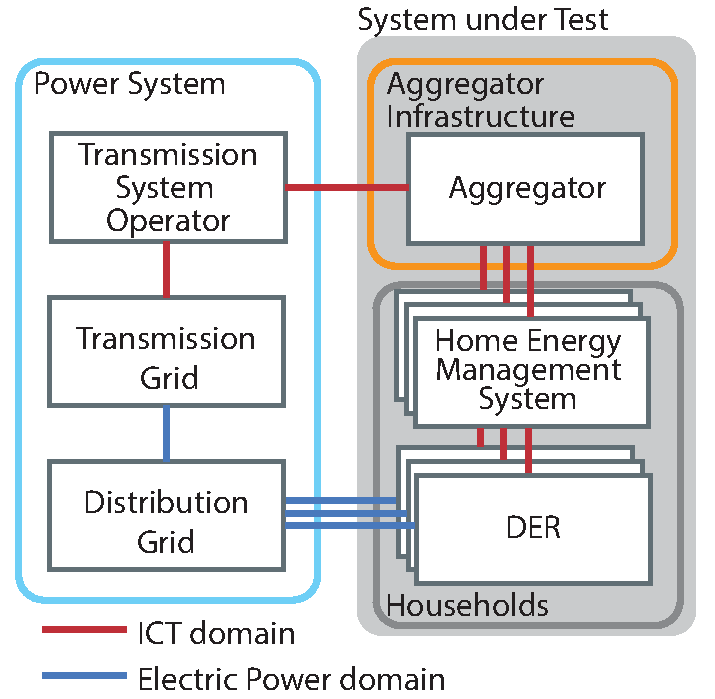
\includegraphics[width=0.75\columnwidth]{figures/example_diagram1.pdf}
\caption{The test setup described by the component centric approach. Note that the aggregator infrastructure and households form the \textbf{SuT}.}% 
\label{fig:examplediagram}
\end{figure}

A sub-test could be a set of physical tests for an aggregator--single household setup, which has as outcome an availability/disturbance model to be used in another (simulation) test setup including a 500 household controller hardware-in-the-loop simulation.


\section{Conclusions}\label{sec:conclusion}
This paper has presented the concept of holistic power system testing to allow for an integrated test of smart grid solutions conducted in different RI.
An approach towards a holistic testing procedure has been proposed.
First results of the approach have been outlined and an exemplification of the outcome given.

In future work, the concepts and definitions will be adapted and refined. The methodological work is strongly interlinked with practical realisation of a holistic testing system and results and experiences will be taken into account in specifying the holistic testing procedure.
A core element is the development of the mapping process from a holistic test to sub-tests and RI that will build on the work presented here.
Concepts from design of experiments will be investigated for coupling results of tests from different RI.



% needed in second column of first page if using \IEEEpubid
%\IEEEpubidadjcol

% An example of a floating figure using the graphicx package.
% Note that \label must occur AFTER (or within) \caption.
% For figures, \caption should occur after the \includegraphics.
% Note that IEEEtran v1.7 and later has special internal code that
% is designed to preserve the operation of \label within \caption
% even when the captionsoff option is in effect. However, because
% of issues like this, it may be the safest practice to put all your
% \label just after \caption rather than within \caption{}.
%
% Reminder: the "draftcls" or "draftclsnofoot", not "draft", class
% option should be used if it is desired that the figures are to be
% displayed while in draft mode.
%
%\begin{figure}[!t]
%\centering
%\includegraphics[width=2.5in]{myfigure}
% where an .eps filename suffix will be assumed under latex, 
% and a .pdf suffix will be assumed for pdflatex; or what has been declared
% via \DeclareGraphicsExtensions.
%\caption{Simulation Results}
%\label{fig_sim}
%\end{figure}

% Note that IEEE typically puts floats only at the top, even when this
% results in a large percentage of a column being occupied by floats.


% An example of a double column floating figure using two subfigures.
% (The subfig.sty package must be loaded for this to work.)
% The subfigure \label commands are set within each subfloat command, the
% \label for the overall figure must come after \caption.
% \hfil must be used as a separator to get equal spacing.
% The subfigure.sty package works much the same way, except \subfigure is
% used instead of \subfloat.
%
%\begin{figure*}[!t]
%\centerline{\subfloat[Case I]\includegraphics[width=2.5in]{subfigcase1}%
%\label{fig_first_case}}
%\hfil
%\subfloat[Case II]{\includegraphics[width=2.5in]{subfigcase2}%
%\label{fig_second_case}}}
%\caption{Simulation results}
%\label{fig_sim}
%\end{figure*}
%
% Note that often IEEE papers with subfigures do not employ subfigure
% captions (using the optional argument to \subfloat), but instead will
% reference/describe all of them (a), (b), etc., within the main caption.


% An example of a floating table. Note that, for IEEE style tables, the 
% \caption command should come BEFORE the table. Table text will default to
% \footnotesize as IEEE normally uses this smaller font for tables.
% The \label must come after \caption as always.
%
%\begin{table}[!t]
%% increase table row spacing, adjust to taste
%\renewcommand{\arraystretch}{1.3}
% if using array.sty, it might be a good idea to tweak the value of
% \extrarowheight as needed to properly center the text within the cells
%\caption{An Example of a Table}
%\label{table_example}
%\centering
%% Some packages, such as MDW tools, offer better commands for making tables
%% than the plain LaTeX2e tabular which is used here.
%\begin{tabular}{|c||c|}
%\hline
%One & Two\\
%\hline
%Three & Four\\
%\hline
%\end{tabular}
%\end{table}


% Note that IEEE does not put floats in the very first column - or typically
% anywhere on the first page for that matter. Also, in-text middle ("here")
% positioning is not used. Most IEEE journals use top floats exclusively.
% Note that, LaTeX2e, unlike IEEE journals, places footnotes above bottom
% floats. This can be corrected via the \fnbelowfloat command of the
% stfloats package.






% if have a single appendix:
%\appendix[Proof of the Zonklar Equations]
% or
%\appendix  % for no appendix heading
% do not use \section anymore after \appendix, only \section*
% is possibly needed

% use appendices with more than one appendix
% then use \section to start each appendix
% you must declare a \section before using any
% \subsection or using \label (\appendices by itself
% starts a section numbered zero.)
%



% use section* for acknowledgement
\section*{Acknowledgment}

This work is supported by the European Community's Horizon 2020 Program (H2020/2014-2020) under project ``ERIGrid'' (Grant Agreement No. 654113). Further information is available at the corresponding website www.erigrid.eu. 

The authors would also like to thank all ERIGrid team members contributing to the development so far.

% Can use something like this to put references on a page
% by themselves when using endfloat and the captionsoff option.
\ifCLASSOPTIONcaptionsoff
  \newpage
\fi



% trigger a \newpage just before the given reference
% number - used to balance the columns on the last page
% adjust value as needed - may need to be readjusted if
% the document is modified later
%\IEEEtriggeratref{8}
% The "triggered" command can be changed if desired:
%\IEEEtriggercmd{\enlargethispage{-5in}}

% references section

% can use a bibliography generated by BibTeX as a .bbl file
% BibTeX documentation can be easily obtained at:
% http://www.ctan.org/tex-archive/biblio/bibtex/contrib/doc/
% The IEEEtran BibTeX style support page is at:
% http://www.michaelshell.org/tex/ieeetran/bibtex/
%\bibliographystyle{IEEEtran}
% argument is your BibTeX string definitions and bibliography database(s)
%\bibliography{IEEEabrv,../bib/paper}
%
% <OR> manually copy in the resultant .bbl file
% set second argument of \begin to the number of references
% (used to reserve space for the reference number labels box)
\begin{thebibliography}{1}

%\bibitem{IEEEhowto:kopka}
%H.~Kopka and P.~W. Daly, \emph{A Guide to \LaTeX}, 3rd~ed.\hskip 1em plus
%  0.5em minus 0.4em\relax Harlow, England: Addison-Wesley, 1999.

\bibitem{SET}
European~Commission, \emph{The European Strategic Energy Technology Plan (SET-Plan) -–  Towards a low-carbon future}, 2010.

\bibitem{SmartGridsPath}
H.~Farhangi, \emph{The path of the smart grid}, IEEE Power and Energy Magazine, vol. 8, no. 1, pp. 18-28, 2010.

\bibitem{SmartGridsRoadmap}
International Energy Agency (IEA), \emph{Technology Roadmap Smart Grids}, International Energy Agency (IEA), Technical Report, 2011.

\bibitem{bruendlinger2015}
R.~Br\"undlinger et al. \emph{Lab tests: Verifying that smart grid power converters are truly smart}, IEEE Power and Energy Magazine, vol. 13, no. 2, pp. 30-42, 2015.

\bibitem{CIGRE}
T.~Strasser et al., \emph{Towards Holistic Power Distribution System Validation and Testing -- An Overview and Discussion of Different Possibilities}, in International Council on Large Electric Systems (CIGRE) Session 2016, Paris, France, 2016.

\bibitem{gnesi2012}
S. Gnesi, M. Tiziana Margaria, \emph{The Testing and Test Control Notation TTCN-3 and its Use}, in Formal Methods for Industrial Critical Systems: A Survey of Applications, Wiley-IEEE Press, pp. 205-233, 2012.

\bibitem{baker2007}  
P.~Baker, et al., \emph{Model-Driven Testing: Using the UML Testing Profile}, Springer, 2007. 

\bibitem{beizer1990}
B.~Beizer, \emph{Software Testing Technique}, 2nd Ed., Van Nostrand Reinhold Co., 1990.

\bibitem{bondy2016procedure}
D.E.~Bondy et al., \emph{Procedure for Validation of Aggregators Providing Demand Response}, in 19th Power Systems Computation Conference (PSCC), Genoa, Italy, 2016.

\end{thebibliography}

% biography section
% 
% If you have an EPS/PDF photo (graphicx package needed) extra braces are
% needed around the contents of the optional argument to biography to prevent
% the LaTeX parser from getting confused when it sees the complicated
% \includegraphics command within an optional argument. (You could create
% your own custom macro containing the \includegraphics command to make things
% simpler here.)
%\begin{biography}[{\includegraphics[width=1in,height=1.25in,clip,keepaspectratio]{mshell}}]{Michael Shell}
% or if you just want to reserve a space for a photo:

% You can push biographies down or up by placing
% a \vfill before or after them. The appropriate
% use of \vfill depends on what kind of text is
% on the last page and whether or not the columns
% are being equalized.

%\vfill

% Can be used to pull up biographies so that the bottom of the last one
% is flush with the other column.
%\enlargethispage{-5in}




% that's all folks
\end{document}